\subsection{Setup}\label{sec:setup}
\note{make introduction}

%The tests are, as mentioned in Section \ref{sec:groupgeneration}, going to be performed on groups with member sizes of 4, 8, 12, 16, 20, and 40, and there are going to be 1000 random generated groups of each size. Throughout these tests we have decided to assign $k$ the size 10. In Figure \ref{fig:setup}, we see the how lists of individual recommendations for a group of size $u$ will be put through an aggregation method before outputting a list of k ranked items.
\begin{figure}[h]
	\centering
	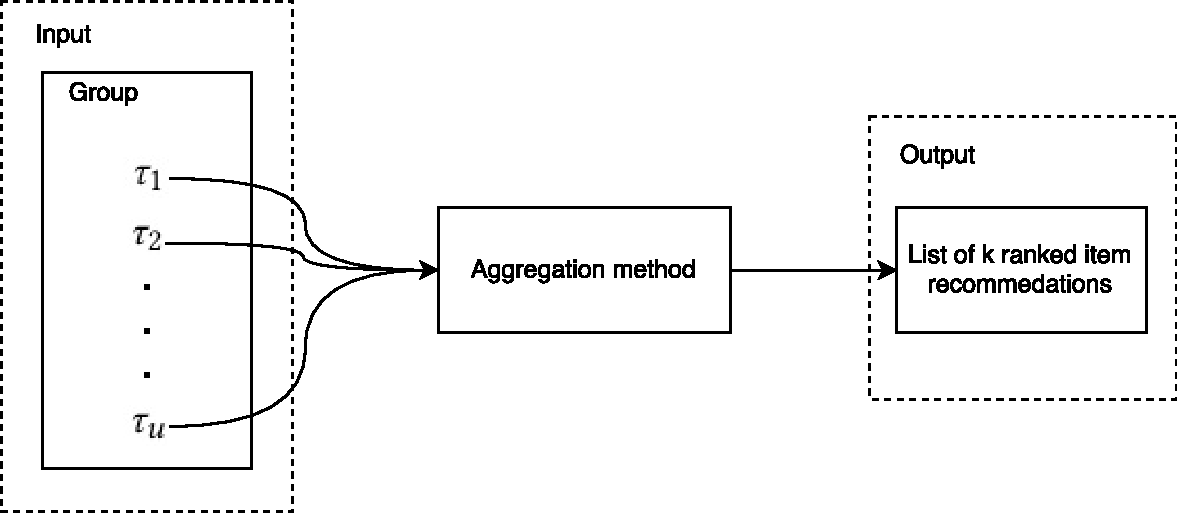
\includegraphics[scale=.4]{graphics/setup}
	\caption{Concept of the test setup. Aggregation methods take in top-k lists and returns a list of recommendations to be evaluated.}
	\label{fig:setup}
\end{figure}
\subsubsection{Dataset}\label{sec:dataset}
We used the MovieLens 100k dataset published by GroupLens in 1998\cite{movielens100k}. MovieLens 100K contains 100.000 ratings between 1 to 5 collected from 943 users across 1682 movies. With room for approximately one and a half million ratings, the 100k rating dataset is sparse. We used rating prediction to populate the rating matrix.

\subsubsection{Individual Recommendations}\label{sec:individualrecommendation}
For rating prediction, we used the library called MyMediaLite\cite{mymedialite}. MyMediaLite is a library for .NET that holds a bundle of recommendation methods for both item recommendation and rating prediction. We will be using the library, because this gives a tested foundation that is easy to reproduce for testing other aggregation methods and the focus of our paper lies in testing the aggregation methods.

Among the methods provided by MyMediaLite, SVD++ is one of the best performing on the 100k dataset on their own records using the parameters in Table \ref{tbl:svdpp}\footnote{www.mymedialite.net/examples/datasets.html}. For the sake of convenience we are using the same parameters as they are proven to be efficient.

\begin{table}[H]
	\centering
	\begin{tabular}{|l|l|}\hline
		Latent Factors & 50 \\
		Regularization & 1	\\
		Bias Regularization & 0.005	\\
		Learning Rate & 0.01 \\
		Bias Learning Rate & 0.07 \\ 
		Number of iterations & 50 \\
		Frequency Regularization & True \\\hline
	\end{tabular}
	\caption{Parameters values for the SVD++ component}
	\label{tbl:svdpp}
\end{table}

\subsubsection{Group Generation}\label{sec:groupgeneration}
For the aggregation we made groups consisting of 4, 8, 12, 16, 20, and 40 users from the MovieLens 100K dataset. This allows us to further the findings by Baltrunas et al\cite{Baltrunas:2010:GRR:1864708.1864733}, who had group sizes from 2 to 8.

Given that the dataset contains 943 users, we limited our group size to 40, as to not have any groups containing more than 5\% of all the users. This ensured some amount of diversity in the group. 40 is also ten times the size of our smallest group, enough to indicate the trend for the quality of recommendations. The groups were created of randomly picked users, and the same user can appear in multiple groups, but never in the same group twice.
\subsubsection{Ranking Measures}\label{sec:ranking}
\note{Make an introduction, old intro was ranking.}
%\subsubsection{Satisfaction Measures}
%\adparagraph{nDCG}

\begin{figure}[H]
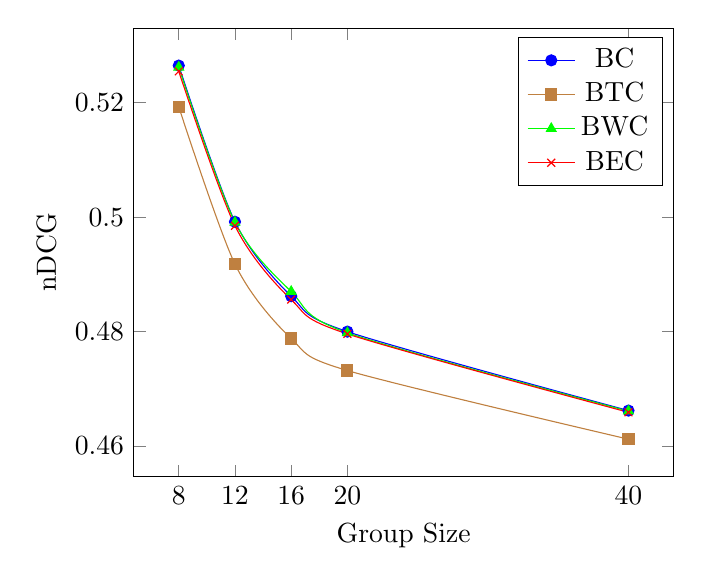
\begin{tikzpicture}
\begin{axis}[
	xlabel=Group Size,
	ylabel=nDCG,
	xtick = {4,8,12,16,20,40}]
		\addplot[smooth,mark=*,blue] plot coordinates {
		%(4,0.6028)
		(8,0.5265)
		(12,0.4992)
		(16,0.4862)
		(20,0.48)
		(40,0.4662)
	};
	\addlegendentry{BC}
	
	\addplot[smooth,color=brown,mark=square*] plot coordinates {
		%(4,0.5995)
		(8,0.5193)
		(12,0.4918)
		(16,0.4788)
		(20,0.4732)
		(40,0.4612)
	};
	\addlegendentry{BTC}
	
	
	\addplot[smooth,color=green,mark=triangle*] plot coordinates {
		%(4,0.6022)
		(8,0.5262)
		(12,0.4991)
		(16,0.487)
		(20,0.4798)
		(40,0.4661)
	};
	\addlegendentry{BWC}
	
	
	\addplot[smooth,color=red,mark=x] plot coordinates {
		%(4,0.6010)
		(8,0.5255)
		(12,0.4985)
		(16,0.4856)
		(20,0.4796)
		(40,0.4659)
	};
	\addlegendentry{BEC}

\end{axis}
\end{tikzpicture}
\caption{Results using nDCG on BC extensions}\label{fig:appendixndcg}
\end{figure}
\subsubsection{Distance Measures}\label{sec:distance}
Before going through the distance measures, we want to cover some general notations that both methods use. As we work with comparing two top-k lists, which are partial lists, we denote them as $\tau_1$ and $\tau_2$. $\tau_1 (i)$ is the notation for the position of element $i$ in $\tau$. $Z = \tau_1 \cap \tau_2$, $z=|Z|$, $S$ is the set of items in $\tau_1$ but not $\tau_2$ and $T$ is vice versa, and $k$ is the length of the top-k lists.

\adparagraph{Kendall Tau Distance}
The idea of Kendall tau distance(KTD) is to compare two ranked lists based on the order in which the items appear. This basically means that it makes pairwise comparisons of item indexes $\{i,j\}$ where $i < j$, so that if $i$ is before $j$ in $\tau_1$ then this should also be the case in $\tau_2$ in order to get a good score. The score is based on a count of how many times $i$ and $j$ are in reverse order. The equation for KTD for complete lists can be seen in Equation \ref{eq:kendalldistancefinal} where $K_1$ and $K_2$ can be seen in Equation \ref{eq:kendalldistance1} and \ref{eq:kendalldistance2} respectively.

\begin{equation}\label{eq:kendalldistance1}
K_1(\tau_1,\tau_2) = | \{(i,j) | i < j, \tau_1 (i) < \tau_1 (j) \land \tau_2 (i) > \tau_2 (j)\}|
\end{equation}
\begin{equation}\label{eq:kendalldistance2}
K_2(\tau_1,\tau_2) = | \{(i,j) | i < j, \tau_1 (i) > \tau_1 (j) \land \tau_2 (i) < \tau_2 (j) \} |
\end{equation}
\begin{equation}\label{eq:kendalldistancefinal}
K(\tau_1,\tau_2) = K_1(\tau_1,\tau_2) + K_2(\tau_1,\tau_2)
\end{equation}

In order to adjust KTD for partial lists we used the $K_{Haus}$ algorithm proposed by Fagin et al\cite{comparing:topk}. This approach has four different cases.

The first case is when both $i$ and $j$ appear in $\tau_1$ and $\tau_2$. In this case the method utilizes Equation \ref{eq:kendalldistancefinal} but only on the items in the set, $Z$.

The second case is when $i$ and $j$ both appear in $\tau_1$ or $\tau_2$ but only $i$ or $j$ appears in the other. Case two is calculated according this formula $(k-z)(k+z+1)- \sum_{i \in S} \tau_1(i)- \sum_{i \in T} \tau_2(i)$. The formula takes the maximum number of items and subtracts the positions from the list containing the items.\note{Revise this explanation, as it is more complex.}

Third case is when $i$ appears in one list and $j$ in the other. For these cases the distance is measured as $(k-z)^2$, which is the disjunctive union of both lists to the power of 2.

The fourth case is when both $i$ and $j$ appear in one list but not the other. In this case Equation \ref{eq:case4} is used. $p$ in this case is a penalty value between 0 and 1. As the method we use is an average approach this value is naturally 0.5. $p$ is multiplied with the binomial coefficient of the length of different items in the top-k lists.

\begin{equation}\label{eq:case4}
2p\left(\!
    \begin{array}{c}
      k-z \\
      2
    \end{array}
  \!\right)
\end{equation}


Combining these cases into one method, we get the $K_{Haus}$ algorithm which can be seen in Equation \ref{eq:khaus}. 
\footnotesize
\begin{equation}\label{eq:khaus}
K_{Haus}(\tau_1,\tau_2) = \frac{1}{2}(k-z)(5k-z+1)+ \sum_{i,j \in Z} K_{i,j}(\tau_1,\tau_2) + \sum_{i \in S}\tau_1(i) - \sum_{i \in S}\tau_1(i)
\end{equation}
\normalsize

The result of the $K_{Haus}$ is normalized by dividing it by $n(n-n)/2$, which gives an approximation of the average distance between the lists. It is an approximation because in case four, the method assumes that there is an equally large chance of the items being in the correct order. Due to this, the method returns 0.78 if the lists are completely disjoint. If the lists are reverse of each other it scores 1 and 0 if the lists are equal. %For a more detail explanation of $K_{Haus}$ go to Fagin et al\cite{comparing:topk} article.

 
\note{Mention somewhere that the results are averages of all group members and all groups}

\adparagraph{Spearman's Footrule Distance}
Another distance measure we use is the Spearman's Footrule Distance(SFD). SFD finds the exact distance between item $i$ in two different ranked lists containing $i$. The way it finds this item distance is by subtracting the item indexes from each other as can be seen in \ref{eq:sfd}. 

\begin{equation}\label{eq:sfd}
F(\tau_1, \tau_2) = \sum_{i=1}^{k} | \tau_1 (i) - \tau_2 (i) |
\end{equation}

As we work with partial lists we use an alternate version called $F_{Haus}$, see Equation \ref{eq:fhaus}, proposed by Fagin et al\citep{comparing:topk}.
As the lists $\tau_1$ and $\tau_2$ can contain different items, the missing index values for items are replaced by $\ell$ which is some value larger than $k$, as it follows that they would be outside the top-k list. Based on the article by Fargin et al we set $\ell$ to be equal to $(3 * k - z + 1)/2$.

\footnotesize
\begin{equation}\label{eq:fhaus}
F_{Haus}(\tau_1,\tau_2)= (k-z)(3k-z+1)+\sum_{i\in Z} | \tau_1 (i) - \tau_2 (i) | - \sum_{i\in S} \tau_1 (i) - \sum_{i\in Z} \tau_2(i)
\end{equation}
\normalsize
% some items will be missing on the lists. In order to handle this we insert $\ell$ which is equal to $(3 * k - z + 1)/2$ placing the item \note{find reason}.  

In order to normalize we divide the result of Equation \ref{eq:fhaus} by $n^2 /2$ which is the maximum value of the algorithm. Doing so we get a value of 0 if $\tau_1$ and $\tau_2$ are in the same order or 1 if the lists are the reverse of each other or completely disjoint.
We made paired t-tests for all methods. Each method is compared with each of the other methods for all measures. The t-test outputs a p-value, which is the probability that the difference between two sets of results is coincidental. At $0.05$ or lower, it is considered that there is statistically significant difference in the means of the two sets.\note{Citation}


%\subsubsection{Ranking Measures}
%To measure our rankings, we use nDCG, Rating nDCG, KTD and SFD, each covered in Section \ref{sec:ranking}. The way we are going to present the results of these tests are by finding an average score for each group. With that we find the average for all the groups, and that is the returned value for the measure.